\newpage
\section{State of the art}

The concept of gadgets might have born with the name of apps in Google's ``Google Personalized Homepage'' in 2005 \cite{ref:what_happened_to_igoogle}, later to be called iGoogle (Figure \ref{fig:igoogle_2008}) and rename these components to gadgets.

\begin{figure}[h]
  \center
    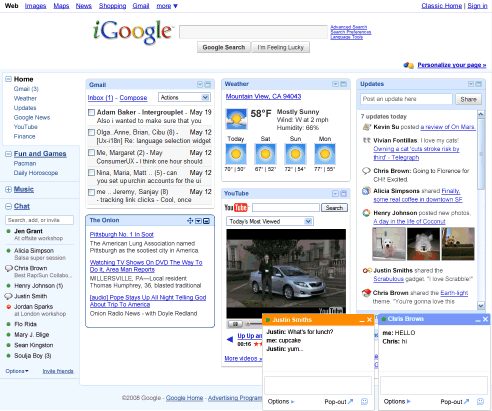
\includegraphics[keepaspectratio, scale=0.6]{Media/Captures/Soa/iGoogle.png}
  \caption{iGoogle in 2008}
  \label{fig:igoogle_2008}
\end{figure}

The social aspect of this apps was being able to share your gadgets with other people, and examples of them would be weather apps, stock apps, video apps...\\[.2cm]
In the latest years of iGoogle's life, before being discounted in 2012, iGoogle apps coexisted with Google Wave, and Google Wave's Gadgets (Figure \ref{fig:wave_gadgets}). This other gadgets offered the advantage of the federated Wave protocol and real-time collaboration \cite{ref:apache_wave_about}.\\[.2cm]
\begin{figure}[h]
  \center
    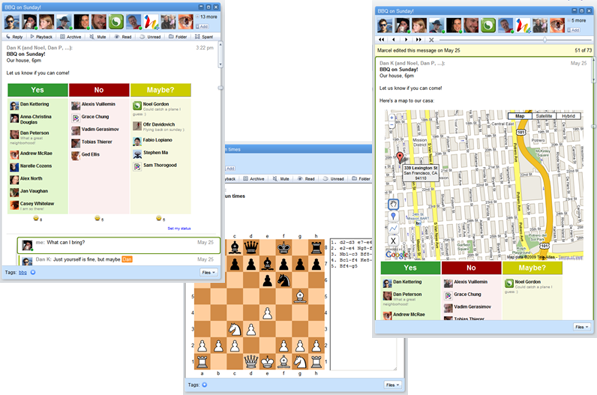
\includegraphics[keepaspectratio, scale=0.5]{Media/Captures/Soa/WaveGadgets.png}
  \caption{Google Wave Gadgets}
  \label{fig:wave_gadgets}
\end{figure}
Then Google began pushing Google+, which can be considered to have some kind of gadgets in the shape of games, which were heavily influenced by Facebook games \cite{ref:facebook_games}, allowing users to play with other people from the same social networks, giving gifts, sharing scores...\\[.2cm]
Google also briefly had Spreadsheet Gadgets, which added unusual functionality for a spreadsheet application in Google Docs.\\[.2cm]
The other aspect explored in this work are robots. Robots usually interact loosely coupled from the software they affect, but as with Wave Gadgets, robots can be incorporated in the main software, acting as an extension to it. An example of this are uNrEaL Bot \cite{ref:unreal_bot}, a collection of robots for very popular video games created to give the user an advantage over the rest of the players, integrating the graphical interface inside the game, and altering the game's own engine.


\begin{center}
------------------------------------------------------------------------------------------\\
\end{center}

\ant{Empieza todas las secciones con una introducción. Continua desarrollando las ideas organizadas temáticamente. Finaliza resumiendo lo que has presentado en la sección e introduciendo la sección siguiente}

\ant{En el state of the art, presenta los trabajos relacionados, indicando las diferencias con tu propuesta.}

\begin{itemize}
  \item Apache Wave Project
  \begin{itemize}
    \item link: incubator.apache.org/wave/
    \item The Apache Wave Project is an incubated project which aims for flexible and dynamic ways of comunication. The main focus of this project is the development of Wave in a Box WiaB, that is a continuation started when Google stopped the development of Google Wave, and tries to complete what Wave was meant to be. The project works towards making reusable components that can be used in other Wave-related products. The project is yet away from reaching a state other than incubation.
  \end{itemize}
  \item Kune
  \begin{itemize}
    \item \anotacion{Am I lying? Where can I find sources for this?}
    \item Kune was originally an independent software, later forked Google Wave to take advantage of its features. Kune keeps now the main Apache Wave's characteristics, but adds a wrapper around giving it a personal space to each user, creative commons licenses to the contents, amongh other extensions.
    \item Kune's main intention is to promote real-time collaboration, as oposed to standard communication, even bidirectional.
  \end{itemize}
  \item Gadgets and robots (Not only wave's)
    \begin{itemize}
      \item Gadgets and robots are present in multiple places of the web space.
      \item Embedded applications
      \begin{itemize}
        \item There are multiple different ways to embed applications or elements in different places of a webpage. In the case of Wave, Google decided to call those elements Gadgets, and Gadgets have outlived Google's Wave and keep being used with the Gadgets API.
        \item The nature of the web nowadays is very reliant on JavaScript [link], and JavaScript makes it easy to embed fully featured applications almost anywhere in a modern browser, as most of them support it [link to support of JavaScript support on different browsers]. But there's other alternatives: Java Applets, Flash components... Wave's Gadgets are JavaScript components inside an iframe.
      \end{itemize}
      \item Robots
      \begin{itemize}
        \item Robots are components on the internet whose objective is to parse content, mainly text [link], and react to it. They can generate reports, gather mass information, notify of events, or even act indistinnguishibly from a common user.
        \item Cons about robots, captchas, robots.txt...
        \item Robots in Kune, they try to avoid the negative aspects of robots
      \end{itemize}
    \end{itemize}
  \end{itemize}  
\end{itemize}
